% ----------------------------------------------------------------------
% ----------------------------------------------------------------------
\section*{Zeitreihen}
Eine Zeitreihe ist eine Folge von Mustern, die nicht mehr isoliert betrachtet werden, sondern bei denen die \emph{zeitliche Reihenfolge} eine wichtige rolle spielt. Damit ist nicht mehr nur das Muster selbst wichtig, sondern auch seine Position in der gesamten Mustersequenz.
Wird eine Zeitreihe mit einem Neuronalen Netz verarbeitet, so hängt die Ausgabe des Netzes nicht mehr nur von der aktuellen Eingabe, sondern auch von den vorangegangenen Eingaben ab.

Die zeitliche Folge der Muster in einem neuronalen Netz kann berücksichtigt werden, indem statt des einzelnen Musters eine Teilfolge von $n$ Mustern gleichzeitig als Eingabe angelegt wird. Dieses Teilfenster wird dann für jedes neue Muster um eine Position nach hinten verschoben. Diese Technik eines beweglichen Fensters (\emph{sliding window}) erlaubt die Verwendung einfacher feedforward-Netze, hat aber folgende Nachteile:

\begin{itemize}
	\item Größe des Fensters ist durch Netztopologie fest vorgegeben.
	\item Nur relative Position innerhalb des Fensters spielt eine Rolle, nicht jedoch die absolute Position in der gesamten Eingabefolge.
	\item Zwei gleiche Teilfolgen der Länge $n$ erzeugen immer die selbe Ausgabe, unabhängig von deren Kontext.
\end{itemize}

Ein anderer Ansatz verwendet \emph{partiell rekurrente Netze}. Diese Netze sind abgeleitet von vorwärtsgerichteten Netzen, besitzen jedoch Rückkopplungsschleifen mit speziell definierten \emph{Kontextzellen}. Solche Kontextzellen realisieren einen Speichermechanismus und leitet ihre Ausgabe an das übrige Netz weiter. So entstehen genau definierte Rückkopplungen.

Diese partiell rekurrenten Netze nehmen eine Zwischenposition zwischen reinen feedforward-Netzen und (vollständig) rekurrenten Netzen wie den Hopfield-Netzen oder der Boltzmann-Maschine ein.
Partiell rekurrente Netze haben den großen Vorteil, dass sie mit geringfügig modifizierten Lernverfahren für feedforward-Netze trainiert werden können, die \emph{effizienter} sind als Lernverfahren für beliebig rekurrente Netze.

Die beiden Techniken der expliziten Repräsentation der Zeit über ein Eingabefenster und der Verwendung partiell rekurrenter Netze, die intern eine Repräsentation der zeitlichen Abfolge bilden können, schließen sich nicht gegenseitig aus, sondern können auch gut miteinander kombiniert
werden.
Einem partiell rekurrenten Netz wird dabei eine Teilfolge von $n$
Mustern gleichzeitig als Vektor präsentiert, diese Teilfolge wird mit der Technik des beweglichen Fensters über die gesamte Eingabefolge geschoben.



% ----------------------------------------------------------------------
% ----------------------------------------------------------------------
\section*{FFNN vs. RNN}
% Quelle: http://minds.jacobs-university.de/sites/default/files/uploads/papers/ESNTutorialRev.pdf
An dieser Stelle soll kurz auf die Unterschiede von \emph{feed-forward neural networks} (FFNNs) und \emph{recurrent neural networks} (RNNs) hingewiesen werden.

Bei FFNNs wird die Aktivierung von den Eingabeneuronen zu den Ausgabeneuronen durchgereicht. Wohingegen RNNs mindestens einen \emph{zyklischen} Pfad von Verbindungen haben. Abbildung \ref{fig:ch04_ffnn-vs-rnn} soll das veranschaulichen.

\begin{figure}[ht!] \centering 
	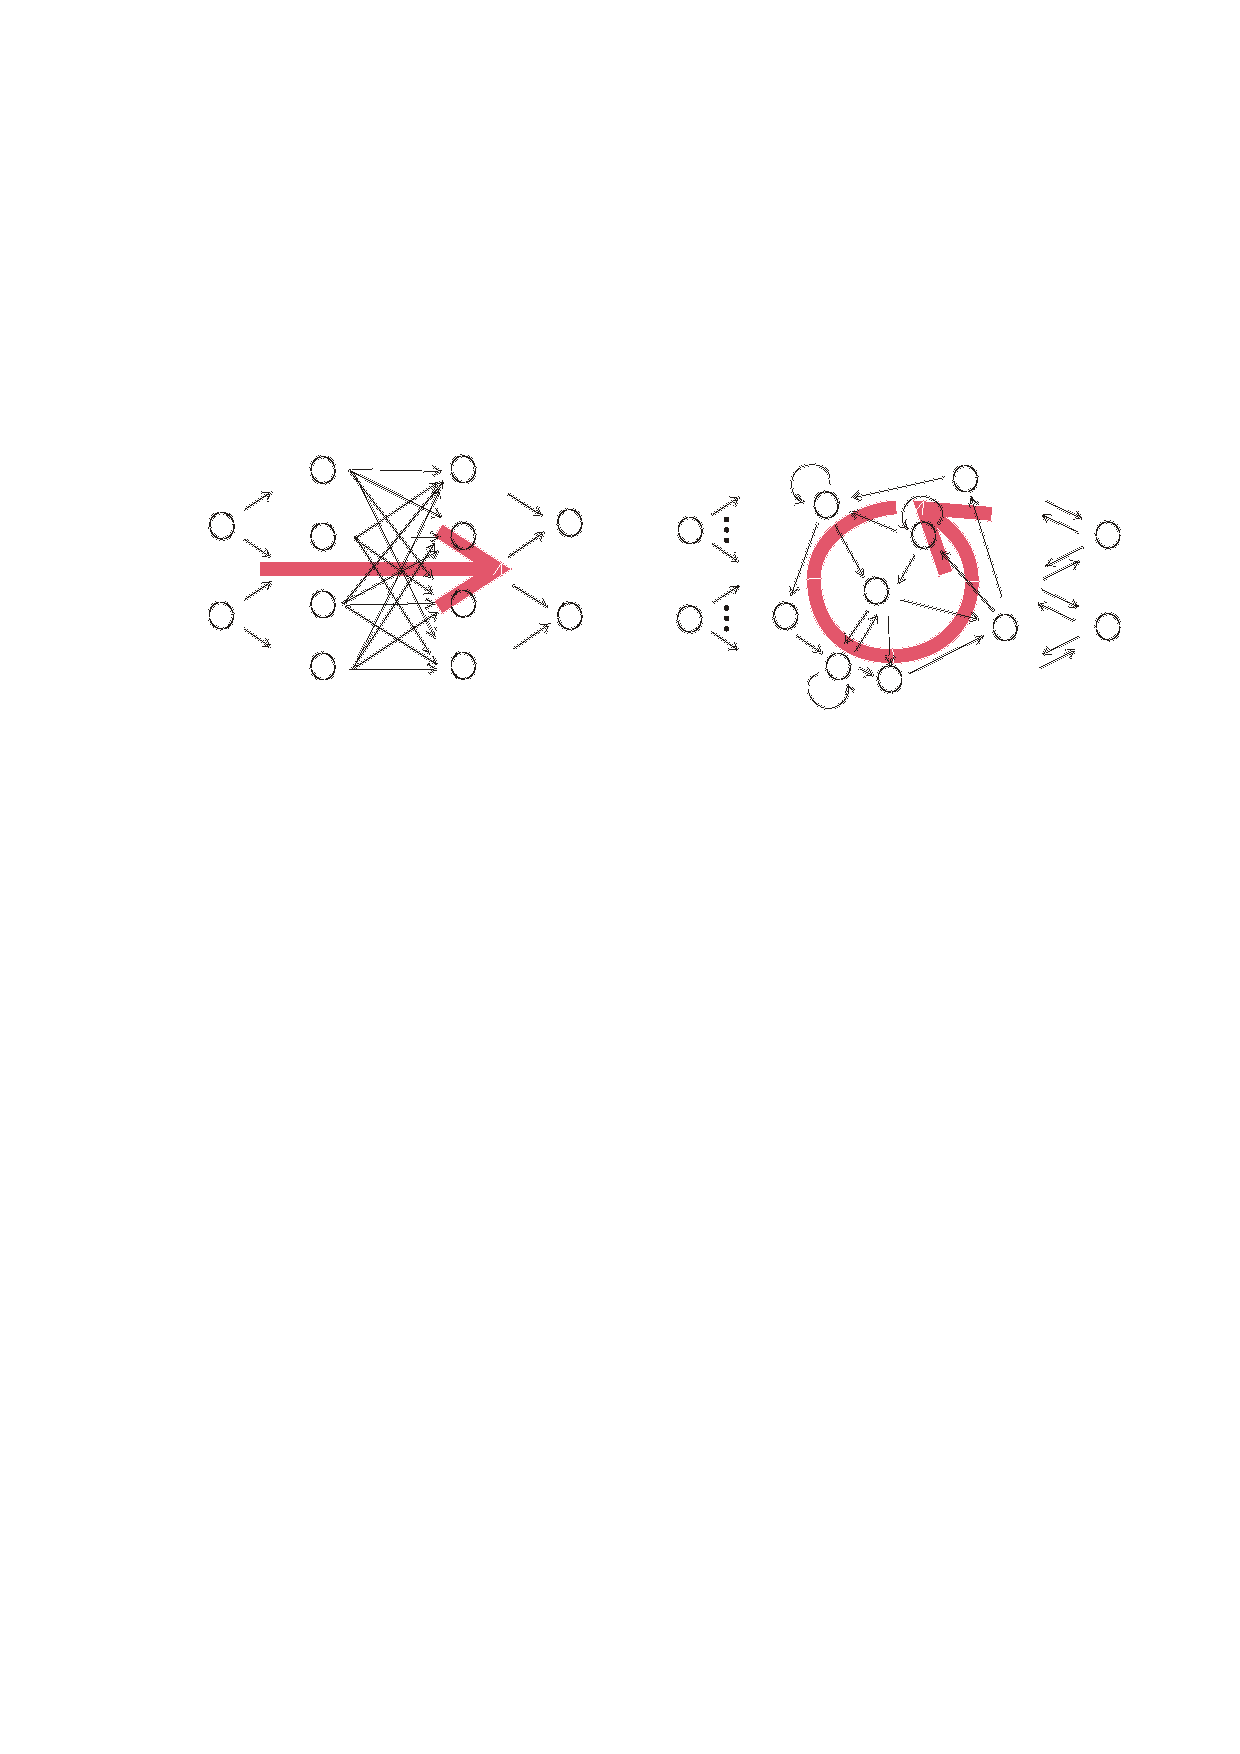
\includegraphics[width=\linewidth]{figures/ch04_ffnn-vs-rnn.pdf}
	\caption{Typische Struktur eines FFNN (links) und eines RNN (rechts).}
	\label{fig:ch04_ffnn-vs-rnn}
\end{figure}

\noindent
Typisch für FFNNs ist:
\begin{itemize}
	\item Typischerweise wird die Aktivierung von den Eingabeneuronen zu den Ausgabeneuronen durch einen oder mehrere versteckte Schichten weitergeleitet (MLP).
	\item Mathematisch gesehen implementieren FFNNs statische Eingabe-Ausgabe-Zuordnungen (Funktionen).
	\item Eignen sich gut als Approximatoren nichtlinearer Funktion und zur Mustererkennung.
\end{itemize}
Typisch für RNNs ist:
\begin{itemize}
	\item Zyklische Aktivierung der Neuronen.  
	\item Mathematisch gesehen implementieren RNNs dynamische Systeme.
	\item Alle biologischen Neuronale Netze sind rekurrent.
\end{itemize}

% ----------------------------------------------------------------------
% ----------------------------------------------------------------------
\section*{Jordan-Netze}
Bei Jordan-Netzen wurde eine Netzarchitektur einfacher feedforward-Netze durch \emph{Kontextzellen} erweitert. Diese Kontextzellen dienen der \emph{Speicherung des Ausgabezustands}.
Eine beispielhafte Architektur ist in Abbildung \ref{fig:ch04_jordan-netze} dargestellt.

\begin{figure}[ht!] \centering 
	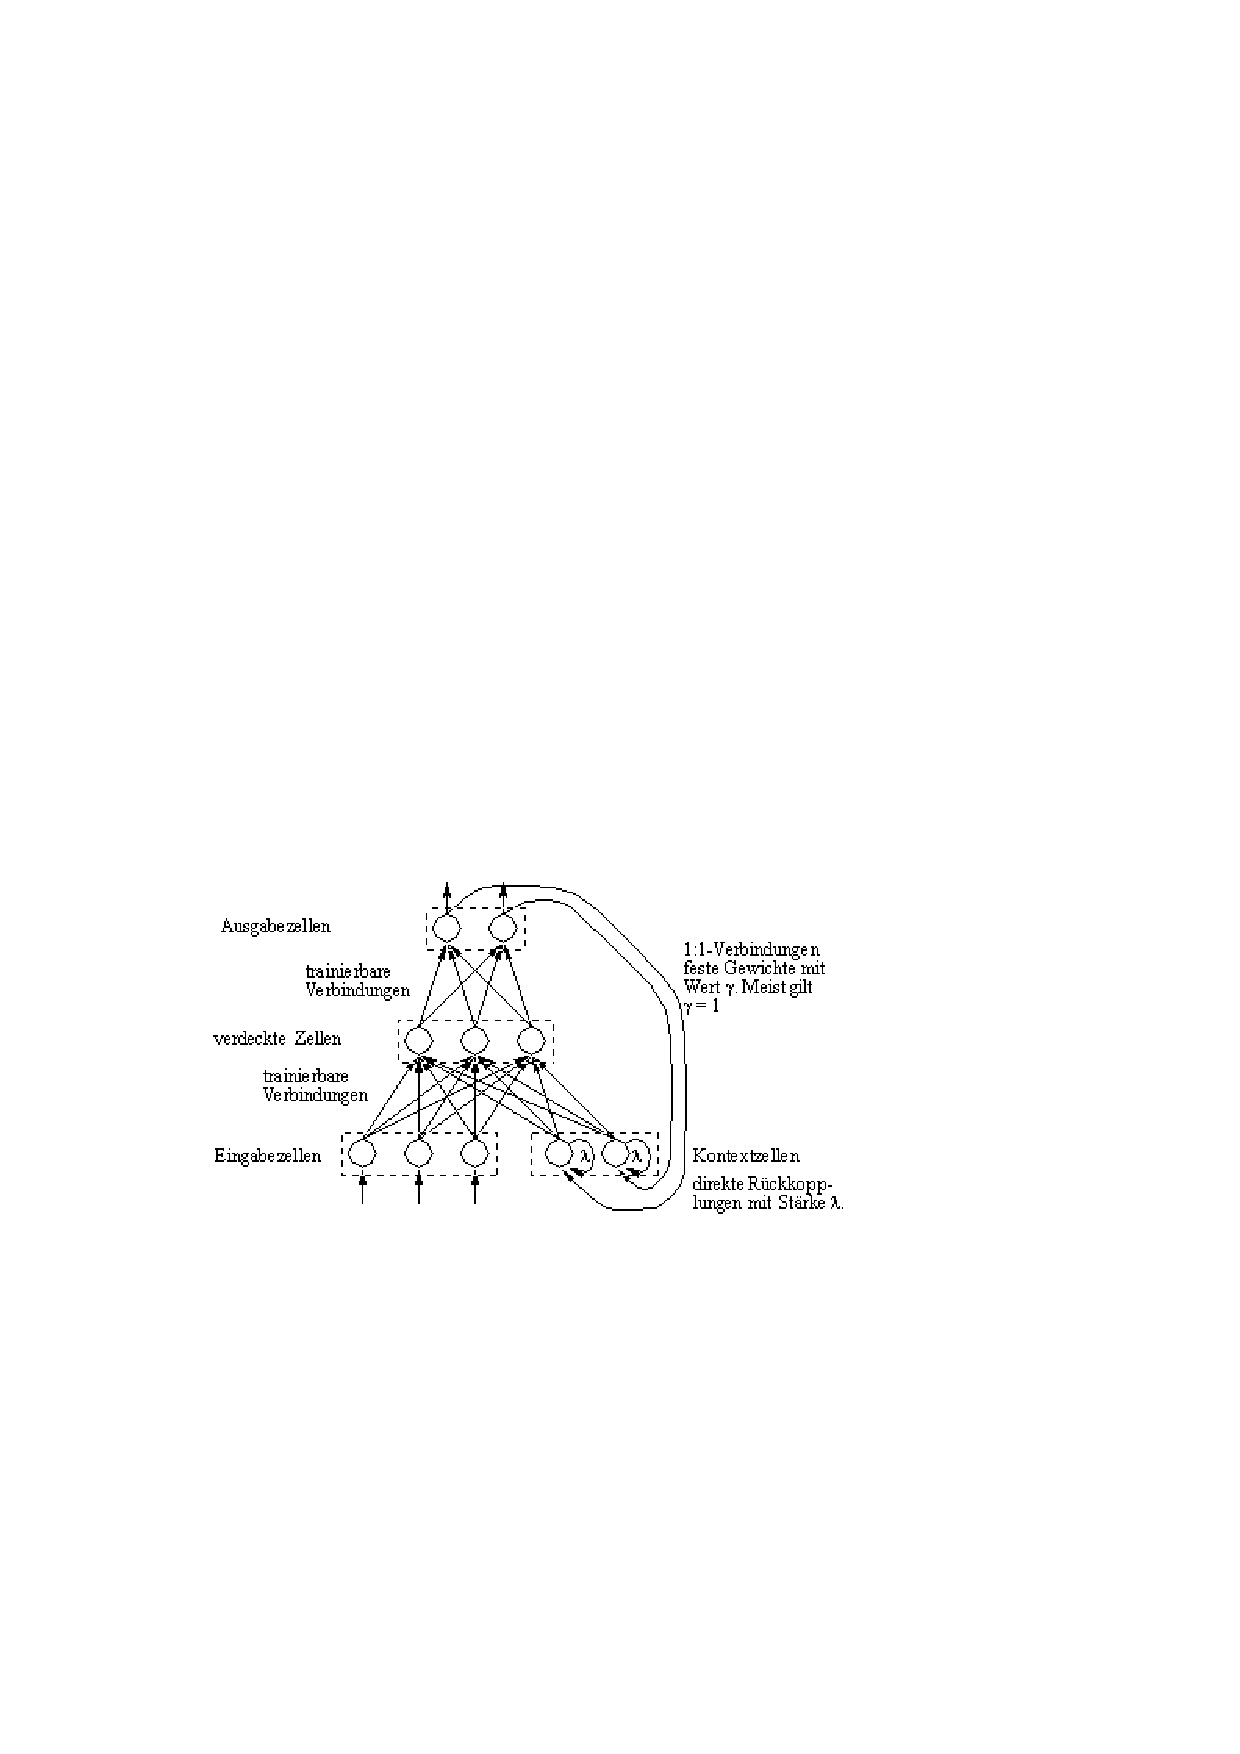
\includegraphics[width=\linewidth]{figures/ch04_jordan-netze.pdf}
	\caption{Architektur eines Jordan-Netzes.}
	\label{fig:ch04_jordan-netze}
\end{figure}

Dabei liefern die Eingabezellen zusammen mit den Kontextzellen die Netzeingabe für die Zellen der verdeckten Schicht. Deren Ausgabe wird an die Ausgabezellen weiterpropagiert und deren Ausgabe wiederum als Netzausgabe zurückgegeben und über 1:1-Rückkopplungsverbindungen mit festen Gewichten als Eingabe an die Kontextzellen weitergegeben.
Die Kontextzellen selbst besitzen direkte Rückkopplungen mit der Stärke $\lambda$, die ebenfalls fest (nicht trainierbar) sind.

Bei dieser Architektur ist zu beachten:
\begin{itemize}
	\item Die Ausgabe der \emph{Ausgabezellen} dient als Eingabe der Kontextzellen
	\item Die Zahl der Kontextzellen muss mit der Zahl der Ausgabezellen übereinstimmen.
	\item Die trainierbaren Verbindungen sind alle \emph{unidirektional}\footnote{Von der Eingabeschicht (incl. Kontextzellen) zur verdeckten Schicht und von dieser zur Ausgabeschicht.} 
\end{itemize}

Für den Fall, dass der Initialkontext der Nullvektor ist und die Rückkopplungsverbindungen von der Ausgabe zu den Kontextzellen alle den Wert $\gamma = 1$ besitzen gilt für den zeitabhängigen inneren Zustand $S(t)$:
\[
	S(t) = \sum_{n=1}^{t-1} \lambda^{n-1} O(t-n)
\]
Wobei $O(t)$ die Netzausgabe zum Zeitpunkt $t$ ist. 



% ----------------------------------------------------------------------
% ----------------------------------------------------------------------
\section*{Elman-Netze}
Elman-Netze sind eine Modifikation der Jordan-Netze, bei der die Rückkopplungsverbindungen nicht mehr von der Ausgabeschicht zur Kontextschicht, sondern von der verdeckten Schicht zur Kontextschicht verlaufen.
Weiterhin entfallen in diesem Modell die direkten Rückkopplungen der Kontextzellen zu sich selbst. Das damit entstehende Modell ist in Abbildung dargestellt.

\begin{figure}[ht!] \centering 
	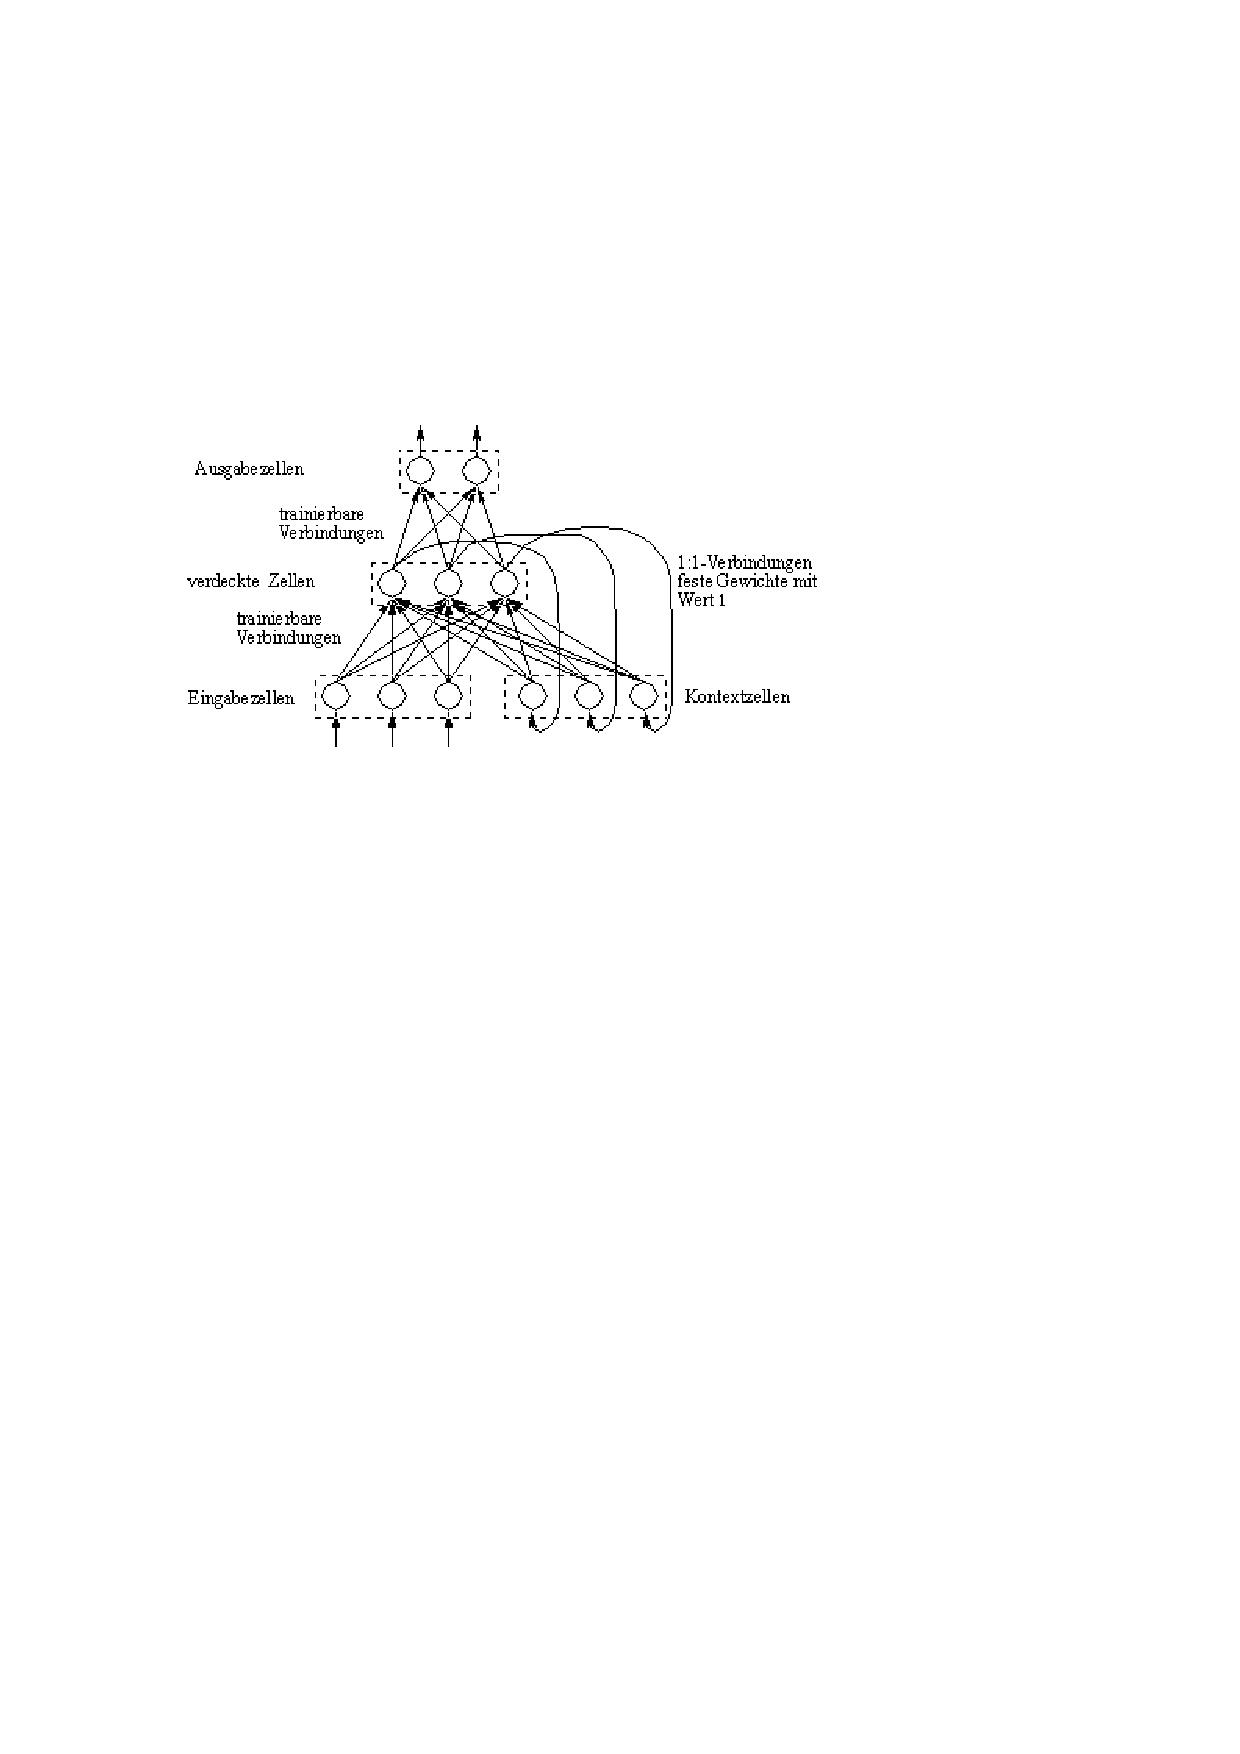
\includegraphics[width=\linewidth]{figures/ch04_elman-netze.pdf}
	\caption{Architektur eines Elman-Netzes.}
	\label{fig:ch04_elman-netze}
\end{figure}

Zu Beginn der Verarbeitung werden die Aktivierungen der Kontextzellen auf einen definierten Wert gesetzt. Nach Eingabe des ersten Musters der Musterfolge werden die verdeckten Zellen sowohl von den Eingabezellen als auch von den Kontextzellen aktiviert.
Da die Kontextzellen die Identität als Aktivierungsfunktion besitzen, ergibt sich der neue Zustand der Kontextzellen als Kopie der Ausgabe der verdeckten Zellen. 
Die verdeckten Zellen geben wie üblich ihre Ausgabe an die Ausgabezellen weiter, die ihrerseits ihre Ausgabe nach außen geben. Dies ist die gesamte Vorwärtspropagierung eines Eingabemusters.
Beim nächsten Eingabemuster enthalten allerdings die Kontextzellen die Aktivierungen der verdeckten Zellen des vorherigen Eingabemusters. Auf diese Weise kann ein zeitlicher Bezug zu früheren Mustern hergestellt werden.

Bei dieser Architektur ist zu beachten:
\begin{itemize}
	\item Die Ausgabe der \emph{versteckten Schicht} dient als Eingabe der Kontextzellen
	\item Die Zahl der Kontextzellen muss mit der Zahl der versteckten Zellen übereinstimmen.
	\item Direkte Rückkopplungen der Kontextzellen existieren nicht.
\end{itemize}

\subsection*{Elman- vs. Jordan-Netze}
Elman-Netze haben gegenüber Jordan-Netzen den Vorteil, dass die Eignung des Netzes für eine bestimmte Anwendung nicht direkt von der zu erzeugenden Ausgabesequenz abhängig ist, wie dies bei Jordan-Netzen der Fall ist. Die internen Zustände ergeben sich vielmehr aus den Zuständen der verdeckten Zellen, sodass diese direkt zu einer Repräsentation des zeitlichen Kontextes gezwungen werden.

\subsection*{Hierarchische Elman-Netze}
Die einfachen Elman-Netze besitzen nur eine verdeckte Schicht Neuronen. Für viele komplizierte Problemstellungen erzielen jedoch Netze mit mehreren verdeckten Schichten etwas bessere Ergebnisse. In diesen Fällen bieten sich hierarchische Elman-Netze an.
Eine beispielhafte Architektur ist in Abbildung \ref{fig:ch04_hierarchische-elman-netze} zu sehen.

\begin{figure}[ht!] \centering 
	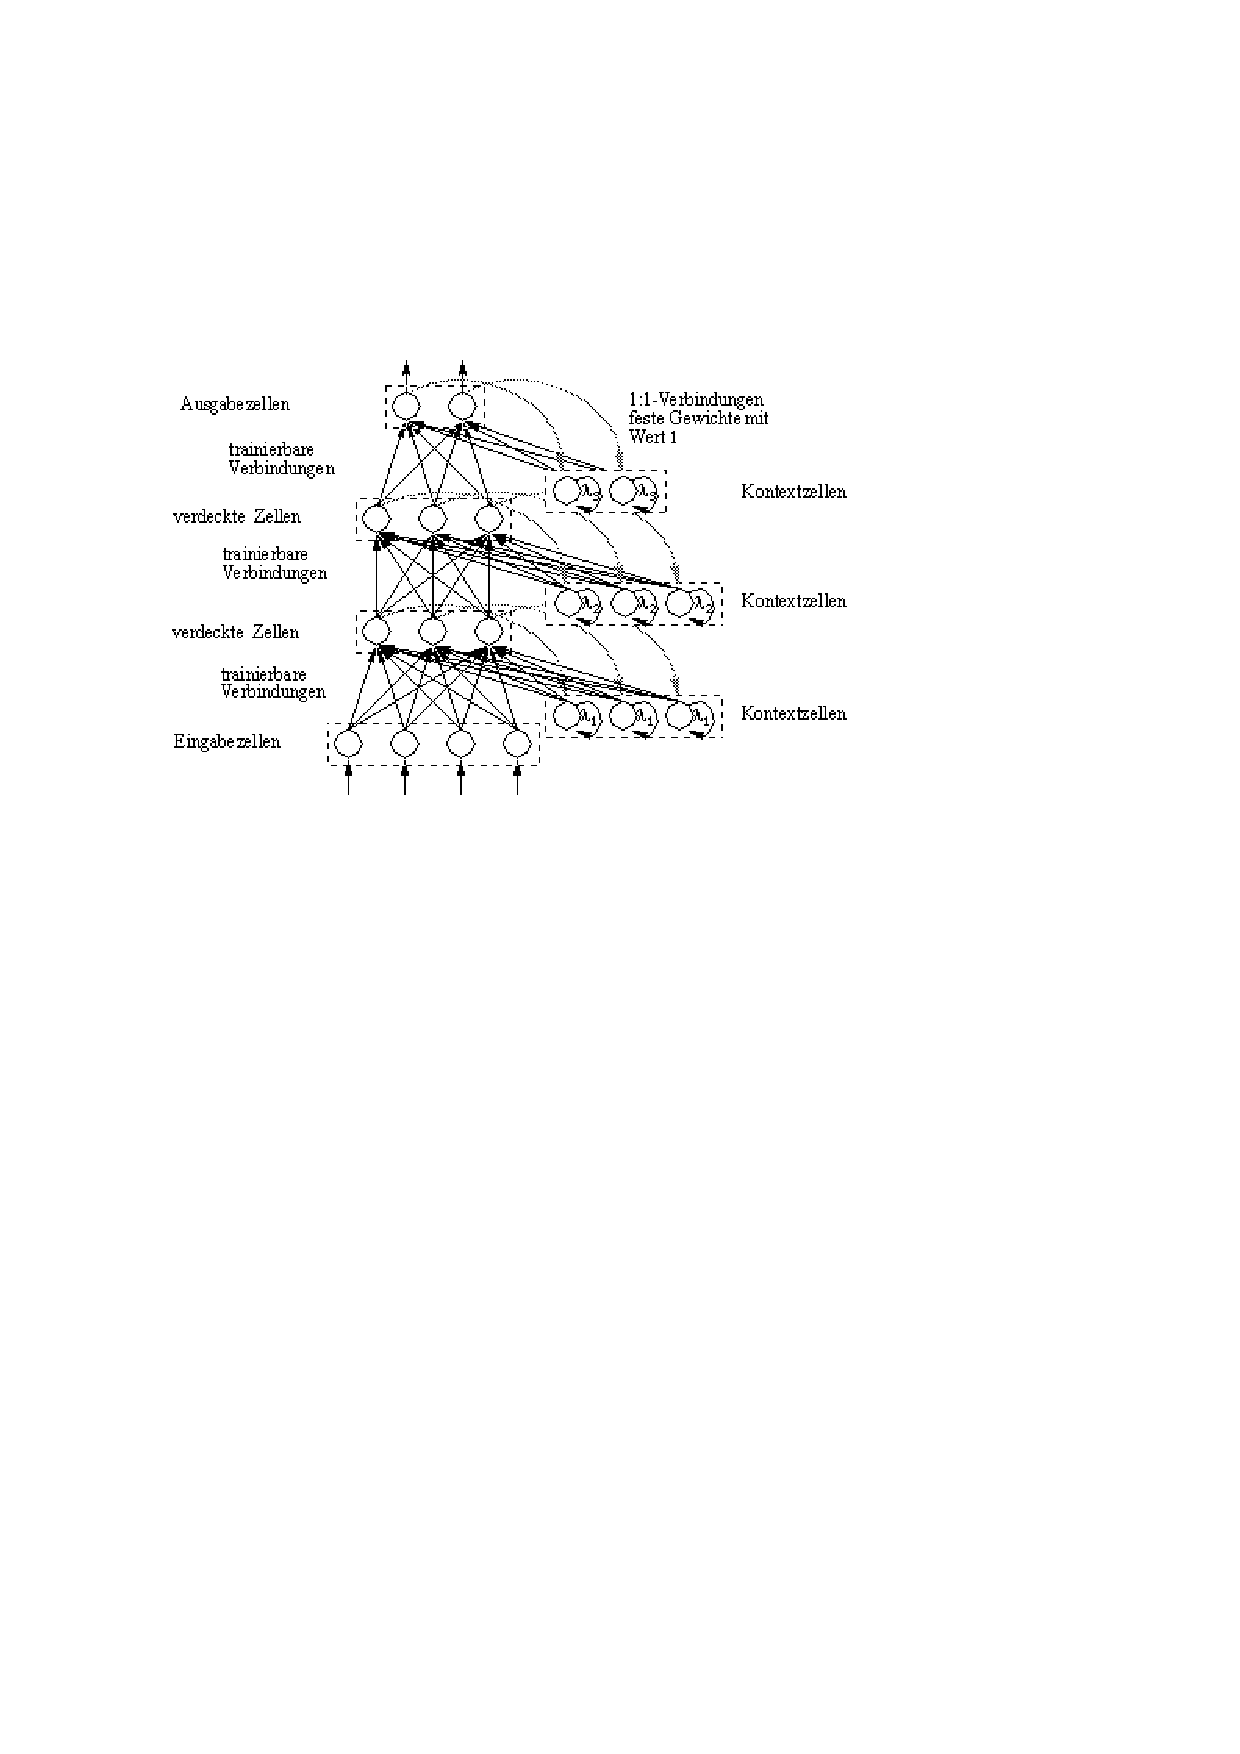
\includegraphics[width=\linewidth]{figures/ch04_hierarchische-elman-netze.pdf}
	\caption{Architektur eines Hierarchischen Elman-Netzes.}
	\label{fig:ch04_hierarchische-elman-netze}
\end{figure}

\subsubsection*{Unterschiede zu Elman-Netzen}
Die Unterschiede zu \textit{normalen} Elman-Netzen sind:
\begin{itemize}
	\item Das Netz hat mehrere verdeckte Schichten.
	\item Auch die Ausgabeschicht erhält Kontextzellen.
	\item Es existieren direkte Rückkopplungen (die Gewichte $\lambda_i$ sind nicht Null). 
\end{itemize}
Die normalen Elman-Netze stellen damit einen Sonderfall der hierarchischen Elman-Netze dar.

\subsubsection*{Vorteile}
Der Vorteil der erweiterten Elman-Netze liegt neben der Existenz mehrerer
verdeckter Schichten vor allem in der Tatsache, dass die Kontextschichten durch die Wahl unterschiedlicher Parameter $\lambda_i$ unterschiedliches Speicherverhalten haben können.



% ----------------------------------------------------------------------
% ----------------------------------------------------------------------
\section*{Lernverfahren partiell rekurrenter Netze}
Partiell rekurrente Netze können mit einer leicht abgewandelten Form des Backpropagation-Lernverfahrens oder verwandten lokalen Fehlerminimierungsverfahren (SuperSAB, Quickprop, RProp) trainiert werden.

Der Schlüssel zu ihrer Anwendung liegt in der Tatsache, dass die Übergangsfunktion, die den neuen internen Zustand beschreibt, durch die Festlegung der \emph{Gewichte der rekurrenten Verbindungen} bereits vor dem Training vollständig definiert wurde und während des Lernens nicht verändert wird.

Lässt man alle rekurrenten Verbindungen im Netz (d.h. alle Verbindungen, die zu Kontextzellen führen) weg, so reduziert sich das Netz auf ein reines feedforward-Netzwerk, bei dem die Kontextzellen einfach zusätzliche Eingabezellen sind.
Der erweiterte Eingabevektor besteht aus dem normalen Eingabevektor und dem Zustandsvektor der Kontextzellen. Der Zustandsvektor der Kontextzellen ist in jedem Schritt durch die feste Übergangsfunktion definiert. Damit kann folgende leichte Modifikation des Online-Backpropagation-Algorithmus für das Training verwendet werden.

\subsection*{Modifikation des Online-Backpropagation-Algorithmus}
Der modifizierte Backpropagation-Algorithmus für Online-Lernen ist im Folgenden aufgeführt. Die mit * markierten Schritte finden unter Nichtbeachtung der rekurrenten Verbindungen statt.

\begin{itemize}
	\item Initialisierung der Kontextzellen
	\item Für jedes Trainingsmuster aus der Musterfolge:

	\begin{itemize}
		\item \emph{Forward Propagation}: Anlegen des Eingabemusters und Vorwärtspropagierung bis zur Ausgabe*
		\item Vergleich der tatsächlichen mit der erwünschten Ausgabe und Berechnung des Fehlersignals für jede Ausgabezelle
		\item \emph{Backward Propagation}: Rückwärtsberechnung der Fehlersignale*
		\item Berechnung der Gewichtsänderung mit Hilfe der Fehlersignale
		\item Adaption der Gewichte
		\item Berechnung des Folgezustands der Kontextzellen gemäß ihrer Eingangsverbindungen (Dies ist der einzige Schritt, bei dem die rekurrenten Verbindungen beachtet werden).   
	\end{itemize}

\end{itemize}

Bei Verwendung des offline-Backpropagation-Algorithmus oder anderer Verfahren, die ein batch-Training erfordern, wie etwa Quickprop, wird der Schritt der Adaption der Gewichte aus der inneren Schleife für jedes Trainingsmuster in die äußere, hier nicht dargestellte Schleife über jede Epoche herausgezogen, sodass die Gewichte nur nach jeder Epoche adaptiert werden.


